\documentclass[UTF8]{ctexart}
\usepackage{amsmath,wrapfig,picinpar,graphicx}
\begin{document}
\thispagestyle{empty}
\pagestyle{empty}

\noindent 如图,直三棱柱 $ABC-A_1B_1C_1$ 的体积为 $4$,$\triangle A_1BC$ 的面积为 $2 \sqrt 2$.

\begin{wrapfigure}{r}{5em}
	\begin{center}
	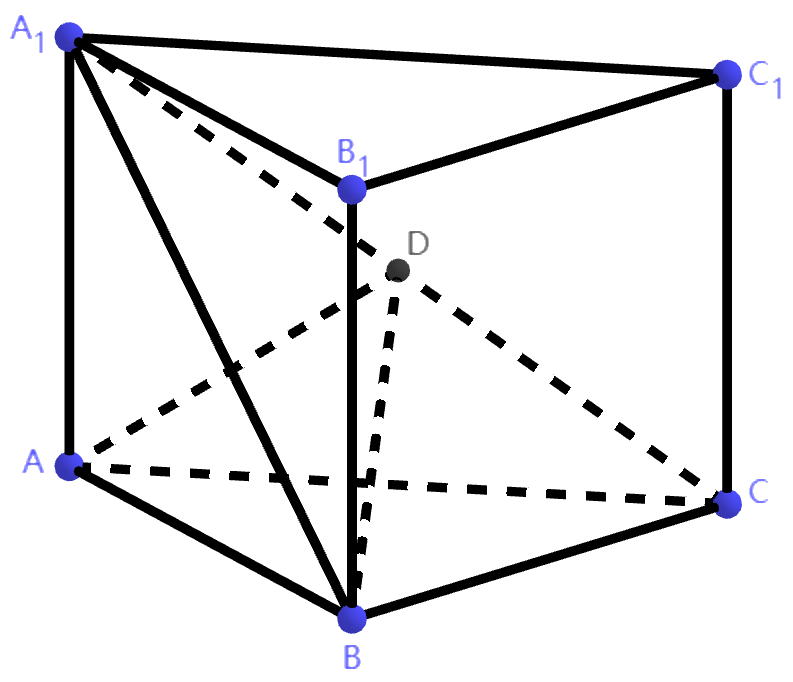
\includegraphics[width=0.5\textwidth]{T19-1.png}
	\end{center}
\end{wrapfigure}

\noindent (1) 求 $A$ 到平面 $A_1BC$ 的距离.

\noindent (2) 设 $D$ 为 $A_1C$ 的中点,$AA_1=AB$,平面 $A_1BC \perp ABB_1A_1$,求二面角 $A-BD-C$ 的正弦值. \\

\noindent 解:(1) $V_{A_1-ABC}=\dfrac{1}{3}V_{ABC-A_1B_1C_1}=\dfrac{4}{3}$. \\

\noindent 则 $h_{A-A_1BC}=\dfrac{3V_{A-A_1BC}}{S_{\triangle A_1BC}}=\dfrac{3V_{A_1-ABC}}{S_{\triangle A_1BC}}=\dfrac{3 \times \frac{4}{3}}{2 \sqrt 2}=\sqrt 2$.

\noindent 故 $A$ 到平面 $A_1BC$ 的距离为 $\sqrt 2$. \\

\noindent (2) 取 $A_1B$ 中点 $E$.

$$\left.
	\begin{array}{rr}
	\noindent AA_1=AB \Rightarrow A_1ABB_1 \text{ 为正方形} \Rightarrow AE \perp A_1B \\
	\text{平面 } A_1BC \cap \text{平面 } ABB_1A_1=A_1B \\
	\text{平面 } A_1BC \perp \text{平面 } ABB_1A_1
	\end{array}
\right\}
\Rightarrow AE \perp \text{平面 }A_1BC.
$$

\begin{wrapfigure}{r}{5em}
	\begin{center}
	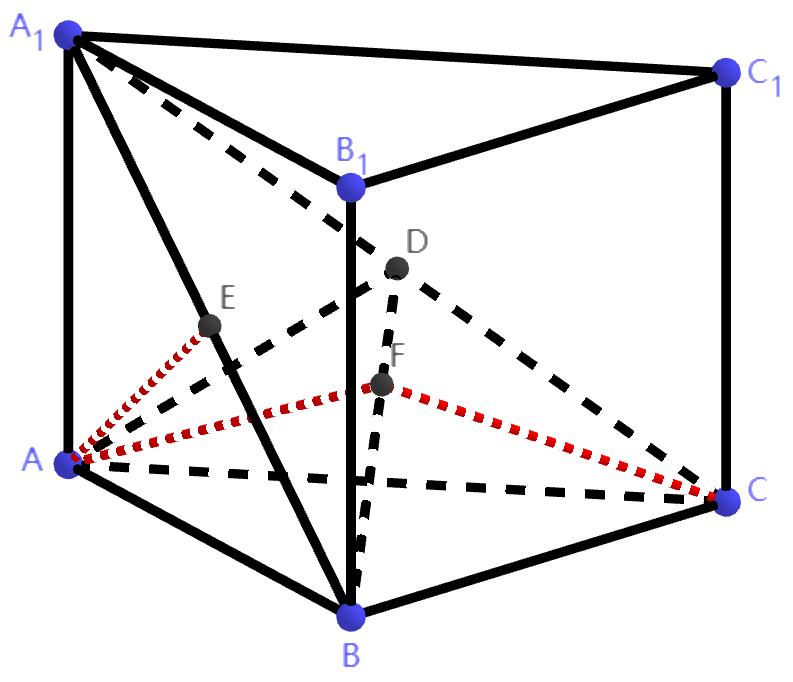
\includegraphics[width=0.5\textwidth]{T19-2.png}
	\end{center}
\end{wrapfigure}

\noindent 又因为 $A$ 到平面 $A_1BC$ 的距离为 $\sqrt 2$,所以 $AE=\sqrt 2 \\
\noindent  \Rightarrow A_1B=2AE=2 \sqrt 2 \Rightarrow S_{\triangle ABC}=\dfrac{V_{ABC-A_1B_1C_1}}{AA_1}=\dfrac{4}{2}=2 \Rightarrow BC=2$.

\noindent 作 $AF \perp BD$ 于 $F$. 则 $\cos \angle ABD=\dfrac{4}{4 \sqrt 3}=\dfrac{\sqrt 3}{3} \Rightarrow BF=\dfrac{2}{3} \sqrt 3, AF=2 \sqrt{\dfrac{2}{3}}=\dfrac{2}{3} \sqrt 6$. \\

\noindent 因为 $\triangle ABD$ 全等于 $\triangle CBD$,所以 $CF \perp BD$. 则 $\sin \angle AFC$ 即为所求.

\noindent 根据余弦定理

$$\cos \angle AFC=\dfrac{AF^2+CF^2-AC^2}{AC^2}=\dfrac{\frac{8}{3}+\frac{8}{3}-8}{2 \times (\frac{2}{6} \sqrt 3)^2}=-\dfrac{1}{2}$$ \\

\noindent 故二面角 $A-BD-C$ 的正弦值为 $\sqrt{1-(-\dfrac{1}{2})^2}=\dfrac{\sqrt 3}{2}$.

\end{document}